\section{Toolkit and Diagnostics}

\tool treats a tokenizer export as an artifact, not as an opaque component of a
trained recommender. The minimum input is a table
\texttt{sid\_assignments(item\_id, sid\_0, ..., sid\_L)}. Optional tables
provide item metadata, interaction histories, and generator outputs. This
contract lets adapters normalize heterogeneous repositories while keeping the
audit independent of a particular training loop. Figure~\ref{fig:audit-sid-pipeline}
shows how heterogeneous exports become comparable reviewer artifacts without
retraining a downstream generator.

\begin{figure*}[t]
\centering
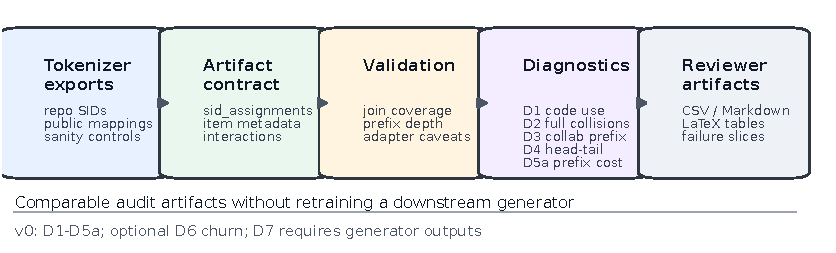
\includegraphics[width=\textwidth]{figures/fig1_audit_sid_pipeline.pdf}
\caption{\tool turns heterogeneous SID tokenizer exports into comparable audit
artifacts. Exports are normalized into a mapping-first contract, validated for
joinability and provenance, and summarized through D1--D5a diagnostics. D6 is
optional churn evidence; D7 is enabled only when generator outputs or beam
traces are provided.}
\Description{Pipeline diagram showing tokenizer exports normalized into
sid assignments, metadata, interactions, optional generator outputs, validation
checks, artifact diagnostics, and generated audit tables.}
\label{fig:audit-sid-pipeline}
\end{figure*}

\paragraph{Artifact contract.}
The contract has three required checks and two optional extensions. The required
checks are: every row must contain a stable item key, every \sid level must be
typed as a discrete token, and the item universe used by diagnostics must be
joinable to the metadata and interaction slices. The optional metadata table
supports semantic or category purity diagnostics. The optional interaction
table supports collaborative-neighborhood diagnostics and head-tail splits.
The optional \texttt{generator\_outputs} table is deliberately separated from
the mapping contract because many public tokenizer releases expose item codes
without trained generator traces.

\paragraph{Validation before metrics.}
\tool refuses to treat an adapter as evidence until it passes coverage and
provenance checks: item-count agreement, missing-code counts, duplicate item
keys, depth consistency, and declared caveats for feature sources or bounded
training runs. This matters for the present resource paper because controlled
exports, sanity tokenizers, and named-method mappings can all be loaded by the
same metric runner but support different claims. The manifest
therefore records whether a row is a runnable named method, a controlled
stressor, an optional extension, or literature-only coverage context.

\paragraph{D1: utilization.}
\tool reports per-level usage, prefix counts, entropy-style imbalance
summaries, and dead or underused code indicators. These expose codebook
collapse and uneven capacity even when full ranking metrics are unavailable.

\paragraph{D2: collision profile.}
\tool measures duplicate full \sid{}s and prefix collisions at each depth. The
reported full-collision rate is the fraction of items whose complete \sid is
shared by at least one other item. In the current resource version, D2 is a
collision profile rather than a causal harm estimate. To make this boundary
visible, the artifact also includes a bounded interaction-qualified controller
inspired by qualification-aware collision work~\cite{hu2026quasid}. The main
metric still reports collisions because full code aliasing is an artifact-level
fact: two items assigned the same complete address cannot be distinguished by a
generator that emits only that address.

\paragraph{D3: semantic-collaborative alignment.}
Semantic grouping and collaborative usefulness need not agree. \tool therefore
computes a co-occurrence-based collaborative neighborhood proxy from training
interactions and asks how often prefix neighborhoods recover each item's top-20
co-occurring neighbors. Metadata purity is retained only as an auxiliary
diagnostic, not as the definition of collaborative quality.

\paragraph{D4: head-tail capacity.}
\tool splits items into popularity buckets and measures whether full \sid
capacity and prefix structure are allocated differently across head, mid, and
tail items. This helps separate genuine tokenizer behavior from simply
restating the catalog popularity distribution.

\paragraph{D5a, D6, and D7.}
D5a reports structural cost proxies: \sid length, level-wise prefix fan-out,
duplicate codes, and trie-like expansion pressure. These are not real generator
serving latencies. D6 computes churn between tokenizer refreshes and is useful for
drift-aware continual-tokenization settings~\cite{feng2026dact}. D7 is an
interface hook for generator behavior, such as invalid paths, next-token
entropy, and duplicate generated candidates; it requires
\texttt{generator\_outputs} and is not claimed by the current evidence.

Identifier foundations and recommender diagnostic frameworks motivate the
resource framing, but they are not runnable tokenizer rows. Table
\ref{tab:method-coverage} therefore focuses on SID artifact facets and marks
which parts are demonstrated in v0.

\begin{table*}[t]
\caption{Paper-facing method/facet coverage. The table separates runnable v0
evidence from literature-motivated facets so that coverage context is not
misread as reproduced tokenizer evidence.}
\label{tab:method-coverage}
\footnotesize
\setlength{\tabcolsep}{3pt}
\begin{tabularx}{\textwidth}{@{}p{0.17\textwidth} p{0.19\textwidth} p{0.14\textwidth} p{0.13\textwidth} Y@{}}
\toprule
Facet & Facet anchors, not all reproduced & v0 status & Diagnostics & Claim boundary \\
\midrule
A. Canonical residual SID & TIGER, GRID, RQ-KMeans & Runnable controlled row &
D1--D5a & Musical demo uses processed feature text; no raw-text
TIGER reproduction. \\
B1. Collaborative / predictability aligned & ReSID, CoST, LETTER, DiscRec &
Runnable bounded row & D1--D5a, D3 & Bounded Musical export; no claim that all
B1 systems are reproduced. \\
B2. Collision / utilization / capacity & QuaSID, AdaSID, CARD, CapsID &
Backlog context & D1, D2, D4 & Coverage only; no faithful named-method result
is reported for these rows. \\
B3. Ranking / retrieval aligned & DIGER, joint search-rec SID & Interface hook
& D3, D5a, D7 & D7 needs generated candidates or beam traces, absent from v0. \\
B4. Bottleneck / interface variants & AsymRec, CapsID, Long SID & Future target
& D4, D5a, D7 & v0 covers structural D5a only, not generator behavior. \\
C. Drift / staleness & DACT, SID staleness & Optional smoke & D6 & Continual
tokenization evidence, not a B-cluster replacement. \\
D. Deployment / search surface & Snapchat SID, unified search-rec SID &
Motivation only & D5a, D7 & No production serving latency or online-impact
claim. \\
R0/control layer & RecList, Elliot, How-to-Index, sanity SIDs, MovieLens smoke &
Controls & D1--D5a & R0 papers are not tokenizer methods; sanity rows test
metric behavior only. \\
\bottomrule
\end{tabularx}
\end{table*}
